\documentclass{article} % For LaTeX2e
\usepackage{nips13submit_e,times}
\usepackage{hyperref}
\usepackage{graphicx}
\usepackage{caption}
\usepackage{subcaption}
\usepackage{url}
\usepackage{multirow}
\usepackage{cite}
\usepackage{amsmath} % Required for Math Stuff
\usepackage{bm}
\usepackage{bbm}
\usepackage{caption}
\usepackage{subcaption}

\newcommand{\specialcell}[2][c]{%
  \begin{tabular}[#1]{@{}c@{}}#2\end{tabular}}

\newcommand{\changespace}[1]{\renewcommand{\baselinestretch}{#1}\normalsize}
\changespace{1.0}


\title{Identification of Songbird Species in Field Recordings}


\author{
Hsiao-Yu Tung \\
%Carnegie Mellon University\\
%\texttt{htung@andrew} \\
\texttt{htung@andrew.cmu.edu} \\
htung \\
\And
De-An Huang \\
%Carnegie Mellon University\\
%\texttt{deanh@andrew} \\
\texttt{deanh@andrew.cmu.edu} \\
deanh \\
\And
Xiao-Feng Xie \\
%Carnegie Mellon University\\
%\texttt{xfxie@cs} \\
\texttt{xfxie@cs.cmu.edu} \\
xfxie \\
\And
Yurui Zhou\\
%\texttt{yuruiz@andrew}\\
\texttt{yuruiz@andrew.cmu.edu}\\
yuruiz \\
\And
Joseph Russino\\
%\texttt{yuruiz@andrew}\\
\texttt{jrussino@rec.ri.cmu.edu}\\
jrussino \\
}

\newcommand{\fix}{\marginpar{FIX}}
\newcommand{\new}{\marginpar{NEW}}

\nipsfinalcopy % Uncomment for camera-ready version

\begin{document}


\maketitle

% \begin{abstract}
% \input{abstract}
% \end{abstract}

\section{Introduction}

It is important to gain a better understanding about the climate and ecological changes in the world. One way to address this is to study seasonal migration patterns in songbird populations, since birds respond quickly to environmental changes \cite{walther2002ecological}.
During migratory periods, many species of songbirds use flight calls, which are species-specific and are distinct from other vocalizations. Therefore, flight calls information can be used to determine the relative abundance of species and is important to understand long-term population trends. Due to costly human effort to collect data about birds in traditional methods, using machine learing (ML) methods to identify bird species from continuous audio recordings has been a hot topic in in recent conference competitions.\footnote{\scriptsize ICML 2013: \href{http://www.kaggle.com/c/the-icml-2013-bird-challenge}{The Bird Challenge}; NIPS 2013: \href{http://www.kaggle.com/c/multi-label-bird-species-classification-nips2013}{
Multi-label Bird Species Classification}; MLSP 2013: \href{http://www.kaggle.com/c/mlsp-2013-birds}{Bird Classification Challenge}} Although there are some recent advances \cite{briggs2013instance,Lasseck13,Massaron13,stattnersong13}, it is still an open ML problem to reliably identify bird sounds in field recordings data due to simultaneously vocalizing birds and various background noise \cite{BriggsMLSP13}.

In this project, we will focus on critical aspects of this problem. We start from some existing classification methods, e.g., \cite{mlsp2,chennovel13,briggs2013instance,Lasseck13,Massaron13,stattnersong13}, adapt components to the data we have, and finally develop a scalable software tool. The total process is divided into four steps. First, Audio data are first preprocessed into spectrograms. The spectrograms are further cleaned by applying background noise reduction and image processing techniques, and connected pixels (acoustic patterns) in the spectrograms are labeled into rectangle segments. Second, features are then extracted and selected from different sources, e.g., file statistics, segment statistics and probabilities, and mel-frequency cepstral coefficients (MFCCs). Third, the classification is then done by using multiple algorithms, e.g., naive Bayes, $k$-nearest neighbors ($k$-NN) \cite{cover1967nearest}, support vector machines (SVM) \cite{cortes1995support}, etc. Finally, we will explore some ensemble methods \cite{rokach2010ensemble,kuncheva2003measures,breiman2001random,breiman1996bagging,freund1997decision,hoeting1999bayesian,read2011classifier} for further exploring some properties on overall performance by combining the predictions of models, as well as facilitating scalability in real-world usages. The software developed for this project will be used by the Carnegie Museum of Natural History, and possibly shared with other land managers, researchers, and educators to enhance the use of flight calls as a method to study the patterns of migratory songbirds.


\section{Related work}

As mentioned in the Introduction, the total process is divided into standard steps of ML components.

The first part is about {\em preprocessing and segmentation} audio data of songbirds. Normally audio files are first processed into grayscale image by applying the Fourier transform using a Hanning or Hamming window of samples with some overlap \cite{Lasseck13, mlsp1}. Only relevant frequency range of the scope of domain interests are kept. The narrowed spectrograms are then treated as graysale images. To reduce the background noise, a {\em median clipping} method can be applied on each frequency band and time frame
% to not only remove most background noise, but also capture the sound feature clearly and precisely \cite{Lasseck13}. An alternative is to apply iterations of a whitening filter
\cite{mlsp1}. A spectrogram can also be processed using a series of sub-processes including Gaussian filtering, local gradient, thresholding, and morphological nosing removal \cite{fodor2013ninth}. The resulting images can be further handled using standard image processing techniques such as dilution and median filter (e.g. using \href{http://scikit-image.org/}{scikit-image}). In \cite{Lasseck13}, neighboring pixels exceeding certain spatial threshold (acoustic patterns) in the spectrograms are labeled into rectangle segments. In \cite{fodor2013ninth}, small segments are discarded and remaining holes are filled. In \cite{mlsp1}, a supervised single-instance single-label classifier is used to label the probability of each pixel as bird sound or noise, and then obtain predicted segementations by applying a threshold.

The second part is about {\em feature extraction and selection}, which can have a large impact on later classification results. In \cite{mlsp1}, segment features are divided into two different categories - ``mask descriptors'' and ``profile statistics''. Histogram of gradients (HOG) have also been used \cite{mlsp1}. In \cite{fodor2013ninth}, features are obtained by applying the template matching function of scikit-image to compute the similarity at the maximum value of the normalized cross-correlation map with templates. In \cite{Lasseck13}, features come from three different sources, i.e., file statistics, segment statistics, and segment probabilities. The template matching in \href{http://opencv.org}{OpenCV library} is applied only on absolute-intensive spectrograms. Many existing work \cite{Stowell_NIPSW13,dufour2013clusterized,chennovel13,Massaron13} considers MFCCs%, which have been proved useful for speech recognition,
as features.  Features can also be extracted using unsupervised deep learning \cite{Mencia_NIPSW13}. Additional methods, e.g., rescaling\cite{mlsp1}, concatenation\cite{dufour2013clusterized}, bag-of-words (BoW) model \cite{Li_CVPR05}, and principal component analysis (PCA) \cite{jolliffe2005principal}, can also be used for feature engineering.

The third part is about {\em classification}. Typical methods include naive Bayes, neural networks, logistic regression, Gaussian mixture model, radial basis function (RBF), decision trees, $k$-NN \cite{cover1967nearest}, SVM \cite{cortes1995support}, etc. Binary classifiers can be turned into multi-class ones by using general strategies, e.g., one-versus-all and pairwise decomposition, to classify instances into multiple classes.
Some existing methods have been used for songbird identification. In \cite{dufour2013clusterized}, a LibSVM is used in a one-versus-all fashion, and best scores have been obtained with C-SVC SVM type and linear kernel function. In \cite{Mencia_NIPSW13}, pairwise SVM, LibSVM, decision trees, and neural networks are used, and the merged SVM and RDT often leads to better results. Mutiple-instance multi-label (MIML) classifiers, e.g., MIML-SVM, MIML-RBF, MIML-$k$NN are considered in \cite{mlsp1}.

Finally, {\em ensemble learning} methods have also been used for combining the predictions of several models. In theory, ensembles have more flexibility in the functions they can represent. Typical methods including gradient boosting (GB) \cite{friedman2001greedy}, random forest (RF) \cite{breiman2001random}, extremely randomized trees (ERT) \cite{geurts2006extremely}, bootstrap aggregating (or bagging) \cite{breiman1996bagging}, Bayesian model averaging (BMA) \cite{hoeting1999bayesian}, and ensemble of classifier chains (ECC) \cite{read2011classifier}. Some of them, e.g., GB \cite{chennovel13}, RF \cite{Stowell_NIPSW13,chennovel13,fodor2013ninth},
ERT \cite{Lasseck13}, have been directly used for songbird identification. There are also some hybrid methods. In \cite{chennovel13}, GB and RF are combined by a simple linear blending method, where the final prediction is given by a linear combination of ensemble predictions, and the combination coefficients are determined by a Lasso and elastic-net regularization of generalized linear model. In \cite{Massaron13}, an ensemble of logistic regression and GB classifiers are considered. In \cite{mlsp2}, an ensemble of classifier chains with RF is applied.

Many classification and ensemble methods can be obtained in \href{http://scikit-learn.org}{scikit-learn library}.

\section{Methods}

\subsection{Preprocessing}

Similar to the methods used in \cite{Lasseck13}, we first convert audio files into spectrogram images, and for each segments we use Hanning windows with 75\% overlap. Notice the case that in a processed grayscale image most area was occupied by the random noise. What we want is to get rid of the background noise completely and increase the contrast between real signal and the background. Given the several different algorithm tested, the median clipping algorithm \cite{mlsp1} works best because it not only removes most background noise, but also capture the sound feature clearly and precisely.

Such a algorithm, though perform well in noise removing and feature capturing, requires large amount of computation because the average and variance of each column of the row need to be calculated. Given the huge size of the processed grayscale image, we need a more efficient algorithm to segment the image. Further experiments is also needed to explore an balance point between noise reduction effectivity and efficiency.

Finally, we apply standard image processing techniques to further reduce the residual noise dot. And then we would use find connected pixels from the image and label the segments, as in \cite{Lasseck13}.

\begin{figure}[p]
    \centering
    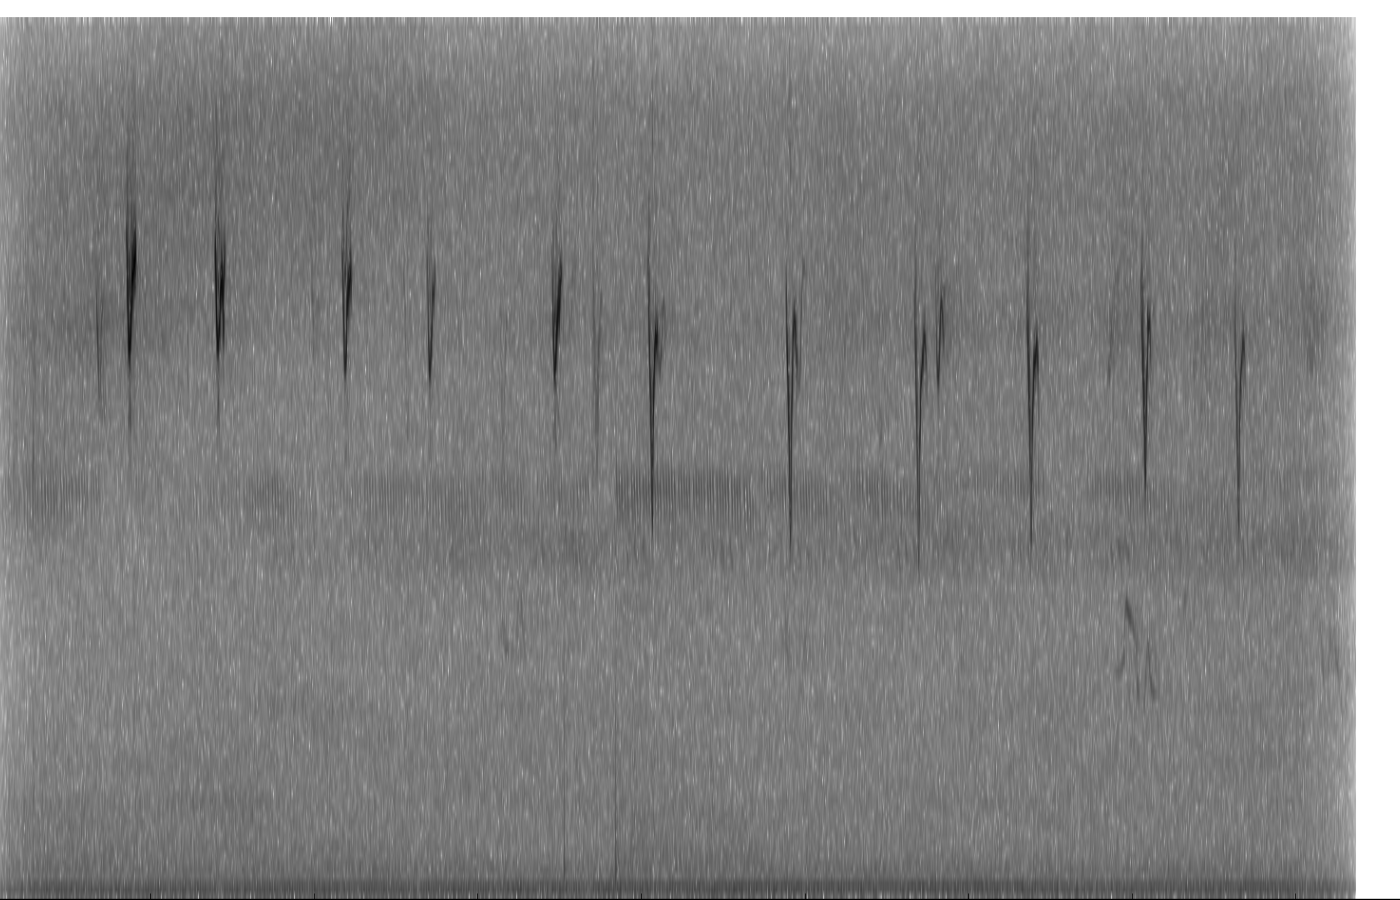
\includegraphics[width=0.8\linewidth, height=0.3\linewidth]{../Figure/Cropped}
     \centering
    \caption{original spectrogram}
    \label{fig:original}
\end{figure}

\begin{figure}[p]
    \centering
    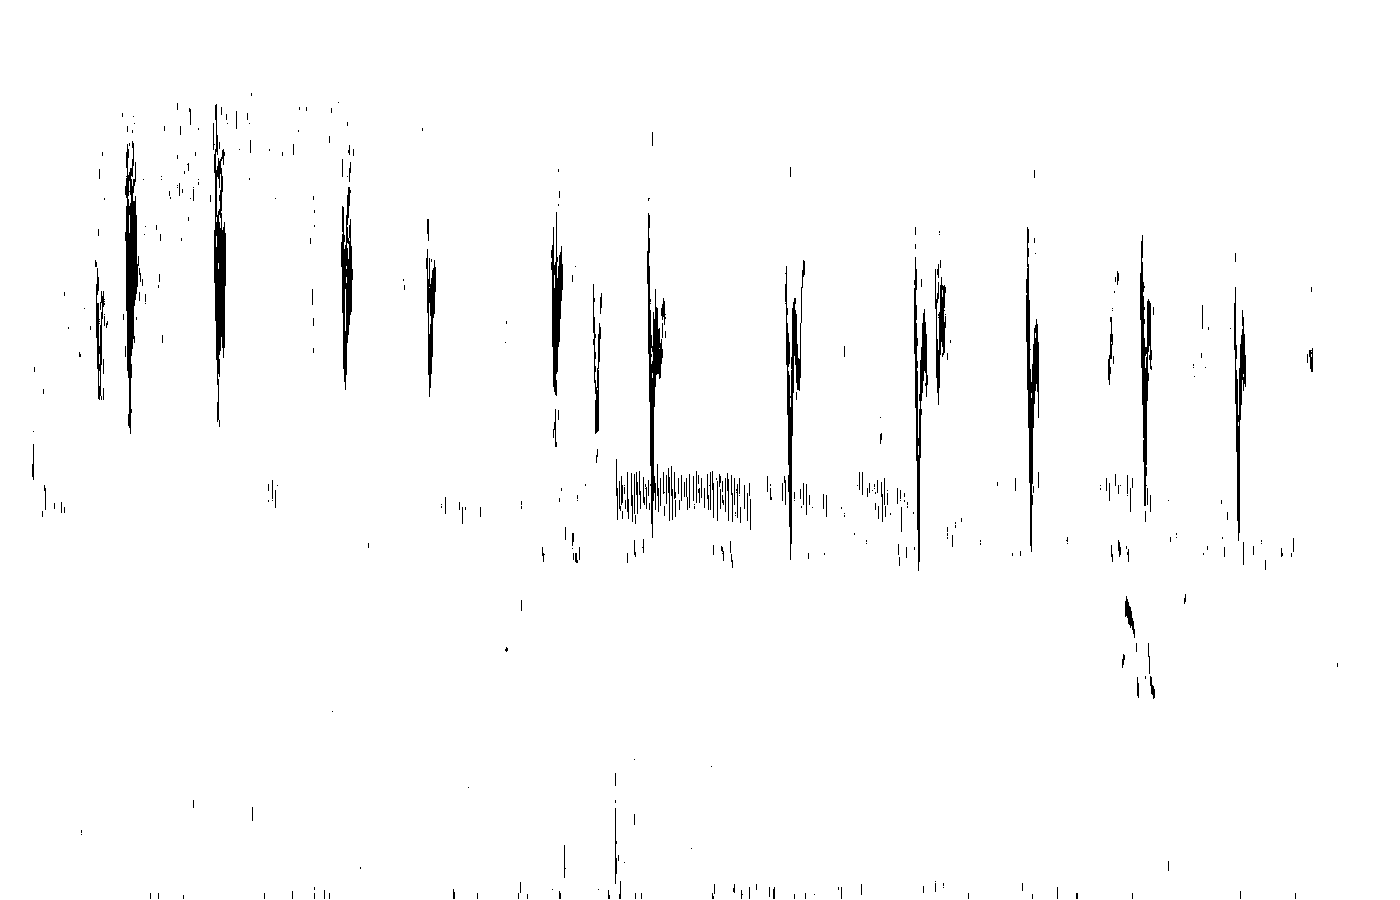
\includegraphics[width=0.8\linewidth, height=0.3\linewidth]{../Figure/Median_clipped}
     \centering
    \caption{Median clipped spectrogram}
    \label{fig:Median_clipped}
\end{figure}

\begin{figure}[p]
    \centering
    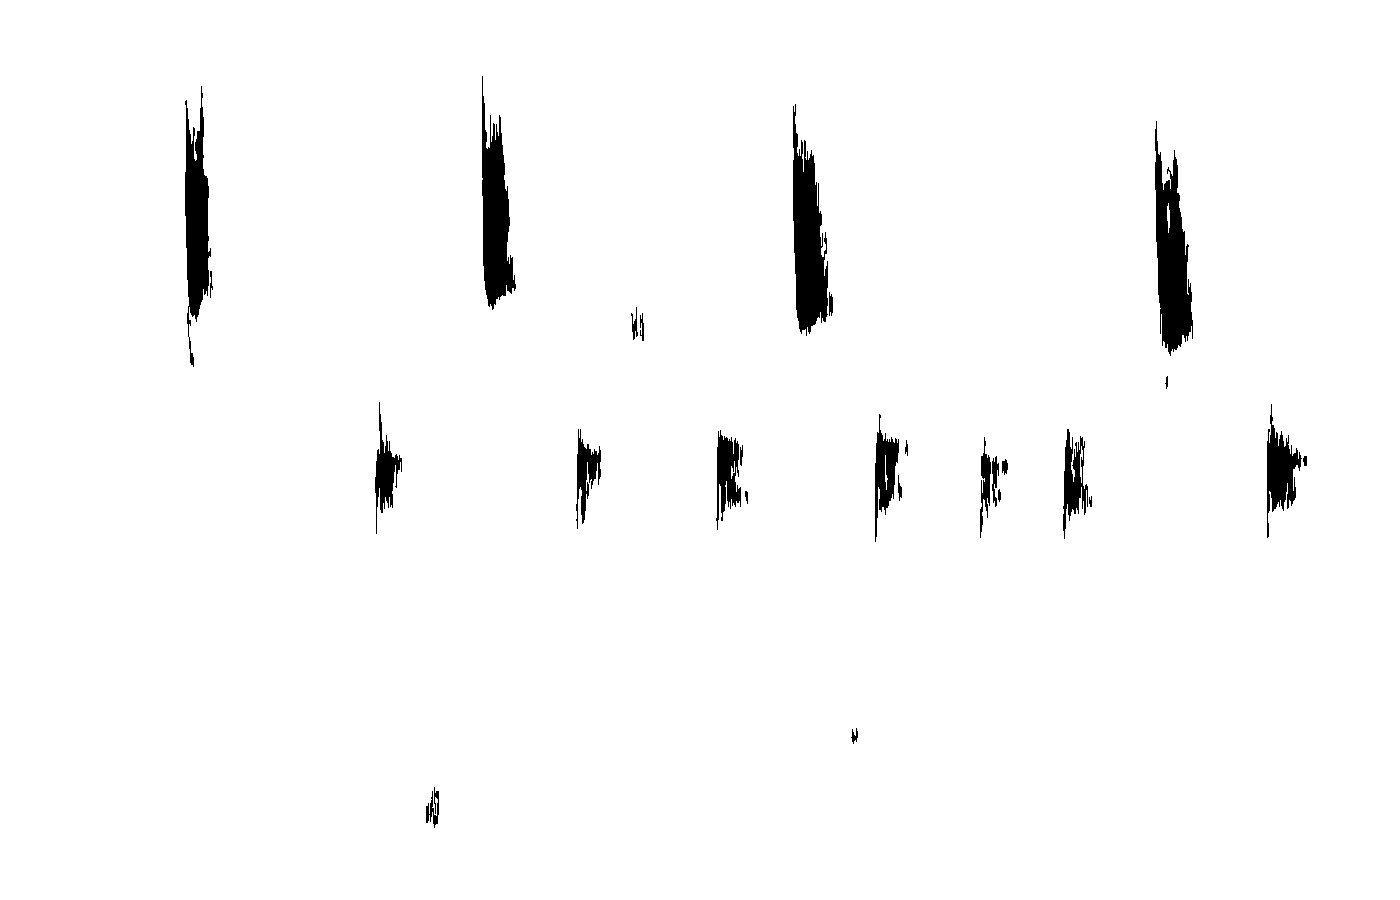
\includegraphics[width=0.8\linewidth, height=0.3\linewidth]{../Figure/Eroded_and_propagated}
     \centering
    \caption{Eroded and propagated}
    \label{fig:Eroded}
\end{figure}

\begin{figure}[p]
    \centering
    \includegraphics[width=0.8\linewidth, height=0.3\linewidth]{../Figure/labeled}
     \centering
    \caption{labeled}
    \label{fig:labeled}
\end{figure}

\subsection{Features}
\label{sec:Features}

\begin{itemize}
	\item Spectrogram based (cite Briggs):
	\begin{itemize}
		\item Mask descriptors: 
		\begin{itemize}
			\item min-$f$, max-$f$, bandwidth (min-max), duration (T)
			\item area, perimeter, non-compactness, rectangularity		
		\end{itemize}
		\item Profile statistics:
		\begin{itemize}
			\item gini, mean, variance, skewness, kurtosis, 
			\item area, perimeter, non-compactness, rectangularity		
		\end{itemize}
		\item Histogram of gradients (HOG)
	\end{itemize}
	\item Mel-Frequency Cepstrum Coefficients (MFCC) based: 
	\begin{itemize}
		\item Has been successful in speech recognition.
		\item 39 dimensional vector. First dimension is energy.
		\item $ T \times 39$ matrix $M$ for each audio file ($T$ is not fixed.)
		\item Continuous features: $\frac{1}{T}\sum_t M_t$, $M_{t_{max}}$, and first PC of $M$
		\item Discretized features: Quantize MFCC by k-means. ($K=200$)
		\begin{itemize}
			\item Bag-of-words: 200-D histogram
			\item N-gram ($N=2,3$): $200^N$-D histogram. Select occurrence $\geq 3$. 
		\end{itemize}
		\item Denoising: Only use $t$ with energy above threshold.	
	\end{itemize}
\end{itemize}




% \textbf{Other features}
% The other features that we intend to explore can be classified broadly into two categories: spectrum-wide features and
% segment features. The spectrum-wide features describe qualities of the full spectrograph for a given recording, while
% the segment features describe qualities of individual segmented portions of the spectrograph. In addition, we plan on using the min, max, average, and standard deviation of frequency values over
% the entire spectrograph, and on dividing the spectrograph into $N$ equally spaced frequency bands and taking the same
% statistics for each frequency band as features. Lasseck had success with this method in 2013 using $N=16$ \cite{Lasseck13}.
%   For segment features, we will use the same basic statistics on a per-segment basis. In addition, we will explore the
% usefulness of many of the other segment features that were used successfully in \cite{mlsp1}. These can be divided
% into two different categories - ``mask descriptors'', which describe the general shape of a segment, and ``profile statistics'',
% which describe the frequency and time profiles within segments. The mask descriptors include bandwidth,duration, area,
% perimeter, non-compactness, and rectangularity; the profile statistics include profile uniformity, mean, variance,
% skewness, and kurtosis. The final set of segment features that we will explore are the Histogram of Gradients (HOG),
% which have successfully been used for songbird classification \cite{mlsp1,fodor2013ninth}.

\subsection{Classifiers}
We consider several classifiers/regressors.

\textbf{Nearest Neighbor (NN).} For each testing data, the NN classifier finds the nearest training data point and transfer the corresponding label. The NN classifier directly reflect the effect of our features and is used as baseline. Depends on the features, different distance metric should be used. We will compare the performance of euclidean and $\chi^2$ distance on the BoW feature in the experiments.

\textbf{Support Vector Machine (SVM).} The most common approach for multi-label classification is to use an ensemble of binary classifiers, where each classifier predicts if an instance belongs to
one specific class or not. SVMs trained in a pairwise fashion has obtained state-of-the-art results on standard multi-label benchmark datasets \cite{Mencia_NIPSW13}. Furthermore, we will be able to integrate different kernels to improve the performance using the SVM. For example, the $\chi^2$ kernel will have a better performance for histogram than the linear kernel. We also consider support vector regression to produce soft output for ensemble learning.

%textbf{Support Vector Regression (SVR).} We use SVR to produce a soft output version of SVM

\textbf{Random Forest.} Random forests has been widely used for multi-label classification \cite{Lasseck13, chennovel13, Stowell_NIPSW13, Zhang_SDM2010}.
Random Forest is operated by constructing decision tree structure by the training examples. One of the popular algorithm is tree bagging, in which the training process includes repeatedly selecting a bootstrap sample of the training set and  fitting the trees to them. After the training process, the label decision is made either on the majority of the votes or a weighted combination from individual trees.

%\textbf{Naive Bayes.}

\textbf{Logistic Regression.} Ensemble of logistic regression has been used for multi-label bird song classification \cite{Massaron13} because of its simplicity. We also consider this method as the baseline for soft output.

\subsection{Ensembles}

An ensemble combines the prediction power of a set of individually trained classifiers $H$ to produce a single classifier. Ensembles often are more accuracy as compared to base classifiers in the ensemble. %For combining the outputs of base classifiers, there are two main types, i.e., weighting methods and meta-learning methods \cite{rokach2010ensemble}. %Popular ensemble methods include Bagging \cite{breiman1996bagging} and AdaBoost \cite{freund1997decision}.

We focus on investigating \emph{weighting} methods, as one of the two main methods discussed in \cite{rokach2010ensemble}, for combining the outputs of base classifiers. Let $M$ be the set of examples, $L$ be the set of labels, $K$ be the set of classifiers, $A_{M*}$ be the true labels, and $A_{MK}$ be the labels assigned by $K$ on $M$. We consider a generalized weighting method. Based on the labels $A_{MK}^\text{train}$ on training examples, weights $W$ and beliefs $B$ are learned, where each $w_k \in W$ is the weight for $k\in K$, and each $b_{l_il_j,k} \in B$ is the belief probability of true label $l_i$, given the label $l_j$ assigned by $k$. For each testing example $X$, the ensemble classifier $\tilde{h}(X)$ assigns votes on labels $L$ by the values $WB$ for testing labels, and return the label or UNKNOWN using majority voting with a threshold value $\bar{V} \in [0, 1]$. 

The weight vector $W$ can be obtained using a \emph{two-step scheme}. First, a subset of top $\tilde{K}$ classifiers are picked with the highest diversity, which has shown to have positive relationship with the ensemble accuracy \cite{kuncheva2003measures}. This result is a binary array $F$. We consider nine measures of diversity \cite{kuncheva2003measures}, i.e., \emph{disagreement}, \emph{correlation coefficient}, \emph{Q-statistic}, \emph{double-fault}, \emph{coincident failure diversity}, \emph{entropy}, \emph{interrater agreement}, \emph{Kohavi-Wolpert}, and \emph{generalized diversity}. Second, weight coefficients $C$ are assigned. The \emph{equal assignment} just gives the same weight as in the canonical majority voting, where the \emph{performance-based assignment} \cite{opitz1996generating} assigns weights proportional to the accuracy performance of each classifier on $M$. The final weights is $W=F\cdot C$.

One can also obtain the weight coefficients $C$ by searching in the configuration space. We consider DEPSO, a cooperative group optimizer \cite{xie2014cooperative}, to obtain the optimal weights for $K$, and thus to know the lowest training error that can be achieved using weights on given $A_{MK}^\text{train}$. Without loss of generality, the weighting space is defined as $c_k\in [0, 1]$ for each weight coefficient on $k$. 

Then we train the belief matrix $B$, by only considering forms that are independent on $k$. A \emph{basic form} of $B$ is a diagonal $L\times L$ sub-matrix for each $k$, which is equivalent to the one using in the canonical majority voting. A \emph{novel form}, which is not included in \cite{rokach2010ensemble}, is to obtain the beliefs as the frequency of $(l_i, l_j)$ pairs, where $l_i=a_{mk} \in A_{Mk}^\text{train}$ and $l_j=a_{m*} \in A_{M*}^\text{train}$, on training examples.

In real-world usages of songbird identification, people would prefer a very higher precision rate, among the classified results on a big amount of testing examples. We accommodate the real-world requirement at the ensemble level, by defining one label as ``UNKNOWN'', to include those instances that are not surely classified. This is also has an implication for scalability, as the labels might change over time, and studies can be mainly performed on ``UNKNOWN'' instances. 

In summary, the generalized weight scheme can be represented by a tuple $<F-learning, C-learning, B-learning>$
%The basic idea is to assign a different weight (function) $w_i$ for each base classifier $h_i\in H$, based on training and true labels on training examples. For each testing instance $X$, the ensemble classifier predicts $\tilde{h}(X)$ outputs the class receiving the highest weighted votes, based on the labels obtained by the base classifiers. 

%\textbf{Bagging} Bagging is an abbreviated term of bootstrap aggregating, which trains each member classifier on a random redistribution of the training set, and using these to get
%an aggregated predictor. It has shown that Bagging is effective on unstable learning algorithms that suffer from significant changes from small perturbations in the learning set.

%Bagging is an averaging method, and the principle is to build several models independently and then to average their predictions.

%\textbf{AdaBoost} AdaBoost is a short name for ``Adaptive Boosting''. AdaBoost can be seen as a broad extension of on-line prediction model in a general decision-theoretic setting. By adapting the multiplicative weight-update rule \cite{littlestone1994weighted}, In theory, boosting can be used to significantly reduce the error of ``weak'' classifiers. AdaBoost is adaptive and can turn weak classifiers into a strong one.

%We will try to exploit the differences between Bagging and Boosting methods: (1) Bagging only uses resampling whereas Boosting uses reweighting; (2) Bagging always uses the uniform distribution whereas Boosting might modify the distribution over examples or mislabels.

%In real-world usages of songbird identification, people would prefer nearly a 100\% precision rate, but can tolerate a  recall rate that is not very high, as the prediction accuracy cannot approach 100\%. Furthermore, scalability is strongly encouraged as the labels (bird species) might change over time. We will accommodate the real-world requirements at the ensemble level, by defining one label as ``UNKNOWN'', and try to improve the precision on all other known labels. 



\section{Experiments}

We first evaluate our system on single-label data to see if the data are separable using our method.

\textbf{Data.}  We use the flight calls of songbirds manually segmented and labeled by Amy Tegeler, an Avian Ecologist from the Carnegie Museum of Natural History, to evaluate the performance of our system on indoor flight calls classification. We used the data from year 2008 to 2013. The total number of species is 32. But only 11 species has more than 100 data. Therefore, the experiment is performed on those 11 species, and 100 data points are randomly sampled from each species. The 100 data points are randomly partitioned into 20 testing data and 80 training data for each species.

\textbf{Segmentation.}
Since the flight call segments are already manually identified, we do not perform segmentation in this experiment.

\textbf{Features.}
We use the Mel-Frequency Cepstral Coefficient, BoW over MFCCs, denoised BoW over MFCCs, 2-Gram and 3-Gram in Section \ref{sec:Features} as the features for this experiment. The size of the code book is 200, and the MFCCs consider the frequencies from 1500 Hz to 22000Hz.

\textbf{Feature Analysis.}
Before beginning with the training process, we first examine the property of the features of BoW over MFCC. We can see that most of the value in the original data is zero. After taking the log value of the data, we can find that a small group of the data is separated from the others (see Figure \ref{fig:hist}). In some of the dimension, this small region contains only a number of specific species of birds, which might be helpful in the classification. 

In the denoised version of BoW over MFCC and 2-Gram features, the features in some of the dimension can clearly separate a specific number of species only by zero and non-zero value. Figure \ref{fig:features} shows the $180^th$ features of denoised BoW over MFCC and the second feature in 2-Gram. In our experiments, we find that the species which can be separated very well by some of the dimensions of these features are classified more accurately than the others. 

\textbf{Feature Selection.}
Due to the limited size of our data, using all the features at the same time will lead to serious overfitting problem. So here feature selection is done by cross validation. After the process, we find that most of the classifiers have higher performance using the denoised version of BoW over MFCC and 2-Gram features. Taking a portion of the features does not help in increasing the performance. To demonstrate the difference between BoW over MFCC and denoised version of BoW over MFCC, we also report the performance of using the former. 

\begin{figure}[b!]
    \centering
    {(a)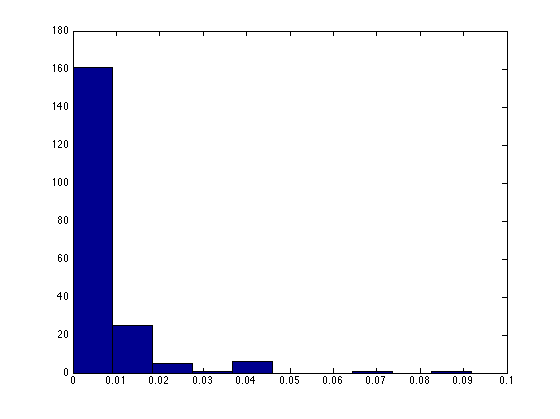
\includegraphics[width=0.40\linewidth]{../Figure/Train_features}
    (b)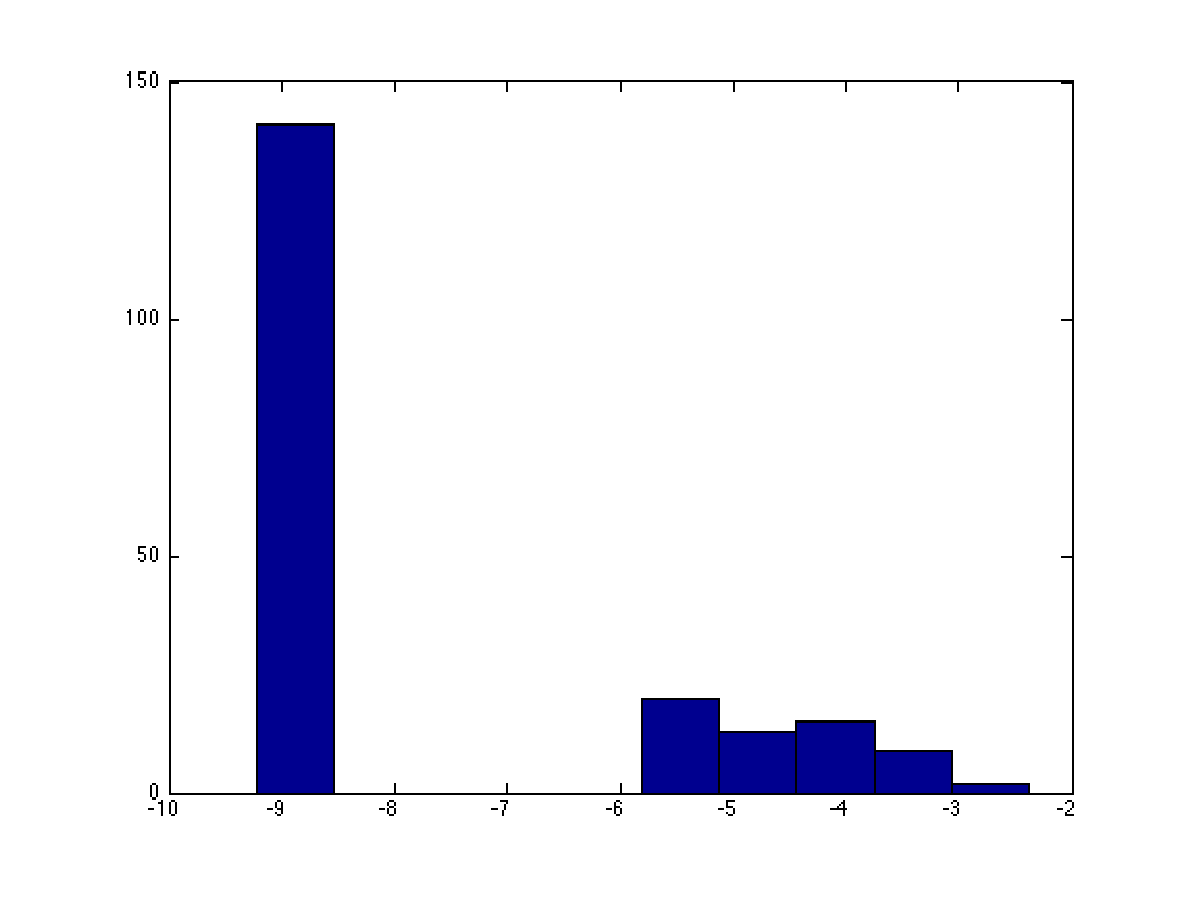
\includegraphics[width=0.40\linewidth]{../Figure/Train_features_log}}
    \caption{(a) is the histogram of second feature. Most of the values are close to zero. (b) is the histogram of the original data after taking log.}
    \label{fig:hist}
\end{figure}


\begin{figure}[b!]
    \centering
    {(a)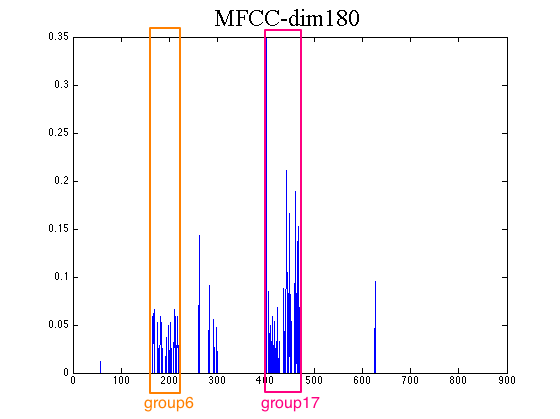
\includegraphics[width=0.40\linewidth]{../Figure/mfcc_180.png}
    (b)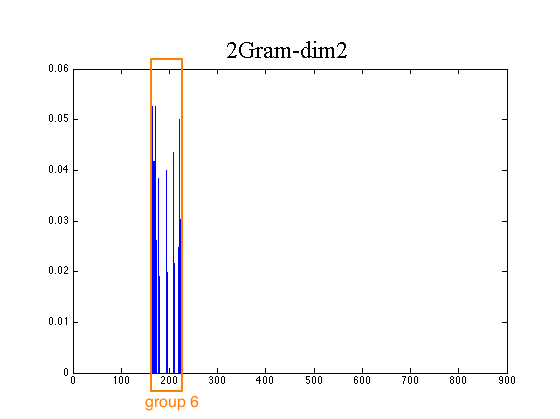
\includegraphics[width=0.43\linewidth]{../Figure/ngram_202.png}}
    \caption{(a) is the $180^th$ features of denoised BoW over MFCC. Most of the high values are around 2 species of birds. (b) shows the second dimension of the 2-Gram features. All the non-zero values appear only whithin one species.}
    \label{fig:features}
\end{figure}
\textbf{Baseline.}
The accuarcy (using Random Forest) on mask descriptors by \cite{mlsp1} is 0.25. 

\textbf{Classifiers.}
In Table \ref{tbl:classifers}, we compare the results using $k$-NN, SVM and random forest classifier. 

First, taking the log over the features of BoW of MFCC decreases the accuracy in rbf SVM classifier. The features are expected to be more of a Gaussian distribution after taking log and can be separated better using rbf kernel. However, the performance decreases. The reason is that the transformed features are distributed in a skrewed Gaussian so that it can not be separated perfectly as well.

Second, the performance of all kinds of classifier increases using the denoised features extracted from BoW of MFCC. Examine the features in images (see Figure \ref{fig:features}) help us understand the properties of them. The denoised features concentrate on a small number of specific species. 

Besides, among all the classifier, SVM classifiers have the highest performance in accuracy and random forest has the lowest performace. The reason why random forest does not perform well on our data is that the sample size is small. SVM with rbf kernel has the highest performance (accuracy: 0.7682) using denoised BoW. The accuracy reaches $0.7818$ with denoised BoW and 2-Gram features. NN has higer performance using chisquare distance with denoised BoW (accuracy: 0.7182).


\begin{table}[t]
\caption{Accuracy of different classifier}
\begin{center}
\label{tbl:classifers}
\begin{tabular}{cccc}
\multicolumn{1}{c}{\bf Classifier }&\multicolumn{1}{c}{\bf Accuracy(\%)}  &\multicolumn{1}{c}{\bf Features} &\multicolumn{1}{c}{\bf Settings}
\\ \hline \\
linear SVM		&67.7273/ 70.4545 		&BoW/ denoised 		&  \\
poly SVM		&69.0909/ 70.4545  	&BoW/ denoised  	& degree: 1  \\
			& 70 			& denoised BoW 	& degree: 2  \\
			& 70.4545  	& denoised BoW 	& degree: 3  \\
rbf SVM       	&70/ 	70.4545  	&BoW/ denoised 		&  \\
                     	&68  			&  BoW (log) 	&  \\
          		&76.8182  		&  denoised BoW 	&  $\gamma = 7.9433$ \\
          		&{\bf 78.1818}  	&  denoised BoW + 2gram 	&    \\
sigmoid SVM     	&70.9091/70.4545	&BoW/ denoised 		&  \\
random forest    	&57/63 			& BoW/ denoised 	& 100 trees; 5 splits \\
       			&63  			& denoised BoW 	& 100 trees; 2 splits \\
NN-euclidean   	&54.09/62.73		& BoW/ denoised 	&  \\
NN-chisquare	&62.27/71.82		& BoW/ denoised 	&  \\

\end{tabular}
\end{center}
\end{table}




\textbf{Ensembles.} Ensemble learning is then performed on the labels by generated 8 classifers, including $k$-NN with euclidean, $k$-NN with chi-square, SVM-linear (-t 0), SVM-$\chi^2$ (-t 5), SVM-RBF (-c 4000 -g 15 -t 2), linear SVM (-c 40), polynomial SVM (-c 1000 -g 1 -d 2 -t 1), sigmoid SVM (-c 1000 -g 1 -d 2 -t 3). We take 4/5 examples as training samples, and 1/5 examples as testing examples.


Figure \ref{fig:diversity_k} gives the training and testing accuracy for the nine measures of diversity (1. \emph{disagreement}, 2. \emph{correlation coefficient}, 3. \emph{Q-statistic}, 4. \emph{double-fault}, 5. \emph{coincident failure diversity}, 6. \emph{entropy}, 7. \emph{interrater agreement}, 8. \emph{Kohavi-Wolpert}, and 9. \emph{generalized diversity}) in different $\tilde{K}$ values, where $C\text{-strategy}$ is uniform, and $B\text{-strategy}$ is the basic form. Accuracy increases as $\tilde{K}$ increases, which might due to $K$ is not sufficently large. However, the test accuracy can be better as
$\tilde{K}=5$ for some measures of diversity.

\begin{figure} [t]
\centering
\begin{subfigure}{.49\textwidth}
  \centering
  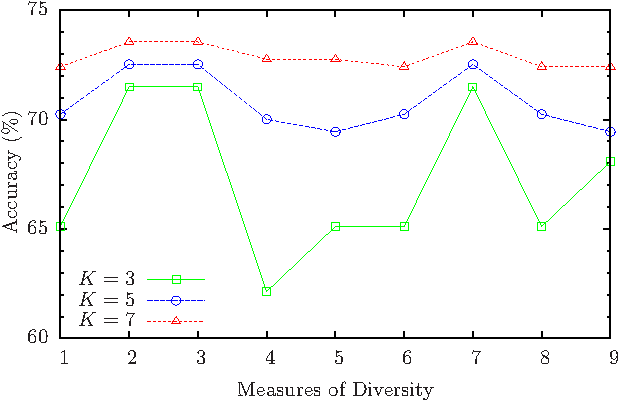
\includegraphics[width=.95\linewidth]{../Figure/diversity_k_train}
  \caption{Training Accuracy}
  \label{fig:diversity_k_train}
\end{subfigure}%
\begin{subfigure}{.49\textwidth}
  \centering
  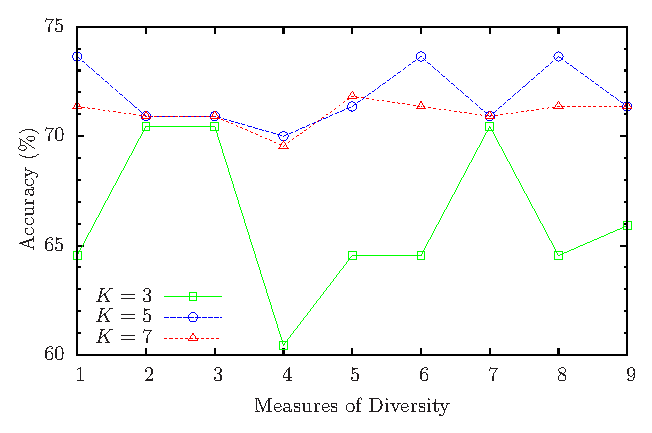
\includegraphics[width=.95\linewidth]{../Figure/diversity_k_test}
  \caption{Testing Accuracy}
  \label{fig:diversity_k_test}
\end{subfigure}
\caption{Training and testing accuracy for different measures of diversity in different $\tilde{K}$ values.}
\label{fig:diversity_k}
\end{figure}

Figure \ref{fig:diversity_0.7_others} gives the training and testing accuracy for different measures of diversity in different $C\text{-strategy}$ and $B\text{-strategy}$, where $\tilde{K}=7$. The new form of $B\text{-strategy}$ can lead to better testing accuracy for some measures of diversity, although does not help on training accuracy.

%Accuracy increases as $\tilde{K}$ increases, which might due to $K$ is not sufficently large. However, the test accuracy can be better as
%$\tilde{K}=5$ for some measures of diversity.

\begin{figure} [t]
\centering
\begin{subfigure}{.49\textwidth}
  \centering
  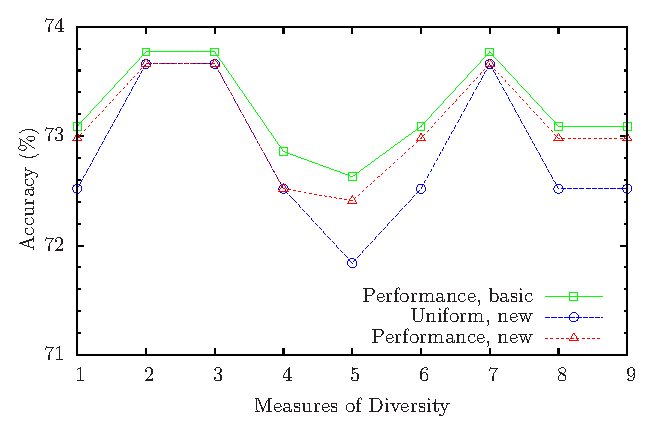
\includegraphics[width=.95\linewidth]{../Figure/diversity_7_others_train}
  \caption{Training Accuracy}
  \label{fig:diversity_0.7_others_train}
\end{subfigure}%
\begin{subfigure}{.49\textwidth}
  \centering
  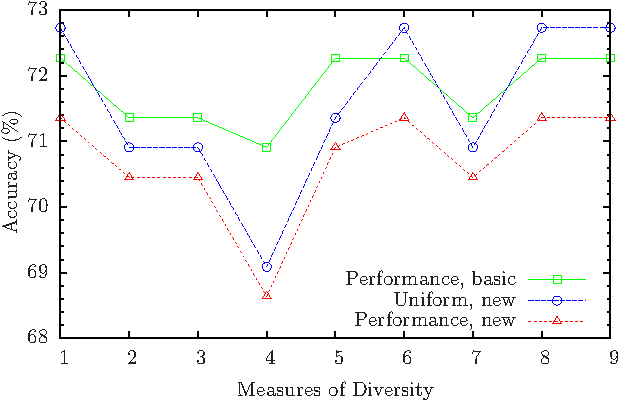
\includegraphics[width=.95\linewidth]{../Figure/diversity_7_others_test}
  \caption{Testing Accuracy}
  \label{fig:diversity_0.7_others_test}
\end{subfigure}
\caption{Training and testing accuracy for different measures of diversity in different $\tilde{K}$ values.}
\label{fig:diversity_0.7_others}
\end{figure}


The search method using DEPSO is performed as $\tilde{K}=|K|$. For the basic and new forms of $B\text{-strategy}$, it respectively obtained 75.26\% and 71.82\% training and testing accuracy, and 75.26\% and 71.36\% training and testing accuracy. This gives the best training accuracy is 75.26\%, and it does not lead to higher test accuracy.

Figure \ref{fig:threshoulds} gives the classification accuracy and rates for different $C\text{-strategy}$ methods in different $\bar{V}$ values, where $\tilde{K}=|K|$, with the \emph{new form} of $B\text{-strategy}$, on testing examples. In general, the accuracy accuracy increases and classification rate decreases, as $\bar{V}$ increases. However, there is a drop at $\bar{V}=0.8$, which means the base classifers may reach agreements on some wrong labels. The optimizion method can keep the classification rate higher, especially in the high accuracy region, which is useful for real-world applications.

\begin{figure} [ht]
\centering
\begin{subfigure}{.49\textwidth}
  \centering
  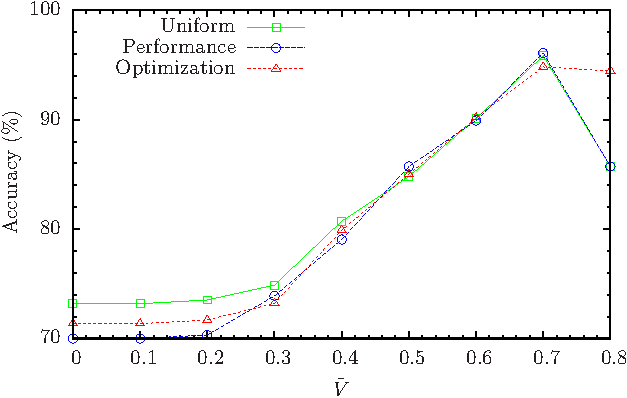
\includegraphics[width=.95\linewidth]{../Figure/threshould_accuracy}
  \caption{Classification Accuracy}
  \label{fig:threshould_accuracy}
\end{subfigure}%
\begin{subfigure}{.49\textwidth}
  \centering
  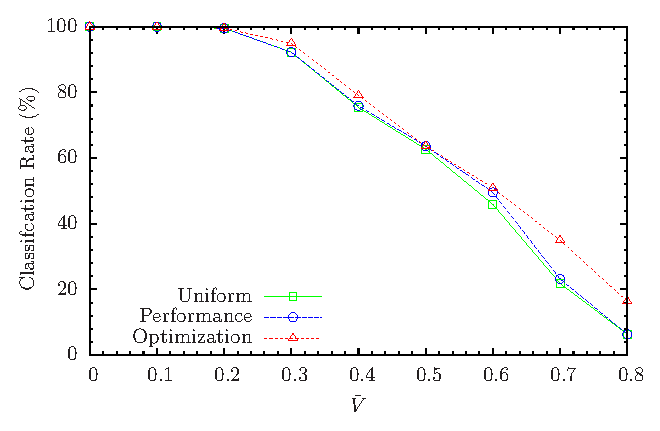
\includegraphics[width=.95\linewidth]{../Figure/threshould_rate}
  \caption{Classification Rate}
  \label{fig:threshould_rate}
\end{subfigure}
\caption{Classification accuracy and rates for different $C\text{-strategy}$ methods in different $\bar{V}$ values.}
\label{fig:threshoulds}
\end{figure}



% \section{Conclusions}
% \input{conclusions}


\bibliographystyle{abbrv}
\bibliography{../bib/birds,../bib/ml}

\end{document}
